\section{Methods \& Materials} \label{methods}
\subsection{Animals}
\textit{Nebria brevicollis}, a species of ground beetle common in the United Kingdom, were collected in the temperate forest around University of Sussex (50\textdegree51'48.8"N, 0\textdegree05'10.9"W) in autumn 2021 (Figure \ref{fig:nebria}). Trapping was done using pitfall traps \citep{Homburg2019}. The beetles were maintained in an incubator at a 12:12h light/dark cycle at 6\degree /11\degree C. The light cycle was shifted 12 hours, so the beetles experiences subjective day during the night, and subjective night during the day. We will just use \textit{day} as \textit{subjective day} hereafter. Beetles were kept individually in plastic containers with soil, sprayed with water and fed one mealworm per week.

% \sidenote{Incubator brand?}

\subsection{Behavioural setup}
For experiments, beetles were placed in a 6-well plate and recorded using an infrared camera. The well plate was illuminated with infrared light from beneath, using a diffusive fabric to diffuse the light. The light source was a desk lamp with a timer. Data collection was done with a Raspberry Pi 4, in a custom written Python software, Bux Recorder. An early version of Bux Recorder synchronised video recordings with environmental logging of light intensity, temperature and relative humidity. The setup frame was built using Makerbeam and custom 3D printed parts. All 3D parts were designed in OpenSCAD, rendered for printing in PrusaSlicer and printed on a Prusa Mini+ 3D printer. All resources are listed in Appendix \ref{tab:resources}.

\subsection{Experimental conditions}
Experiments were carried out between January and May 2022. In each experiment, beetles were observed during a 24 hour period. Three different light conditions were used: Abrupt light/dark (LD) where they were exposed to approximately 6 hours light, 12 hours darkness and 6 hours of light with abrupt changes between light intensities; light/light (LL) 24 hours in light; dark/dark (DD) 24 hours in darkness (Figure \ref{fig:light-conditions}). Each animal experienced all conditions twice with at least 2 weeks between trials.

\begin{figure}[t!]
    \centering
    \begin{subfigure}[t]{0.4\linewidth}
        \caption{}
        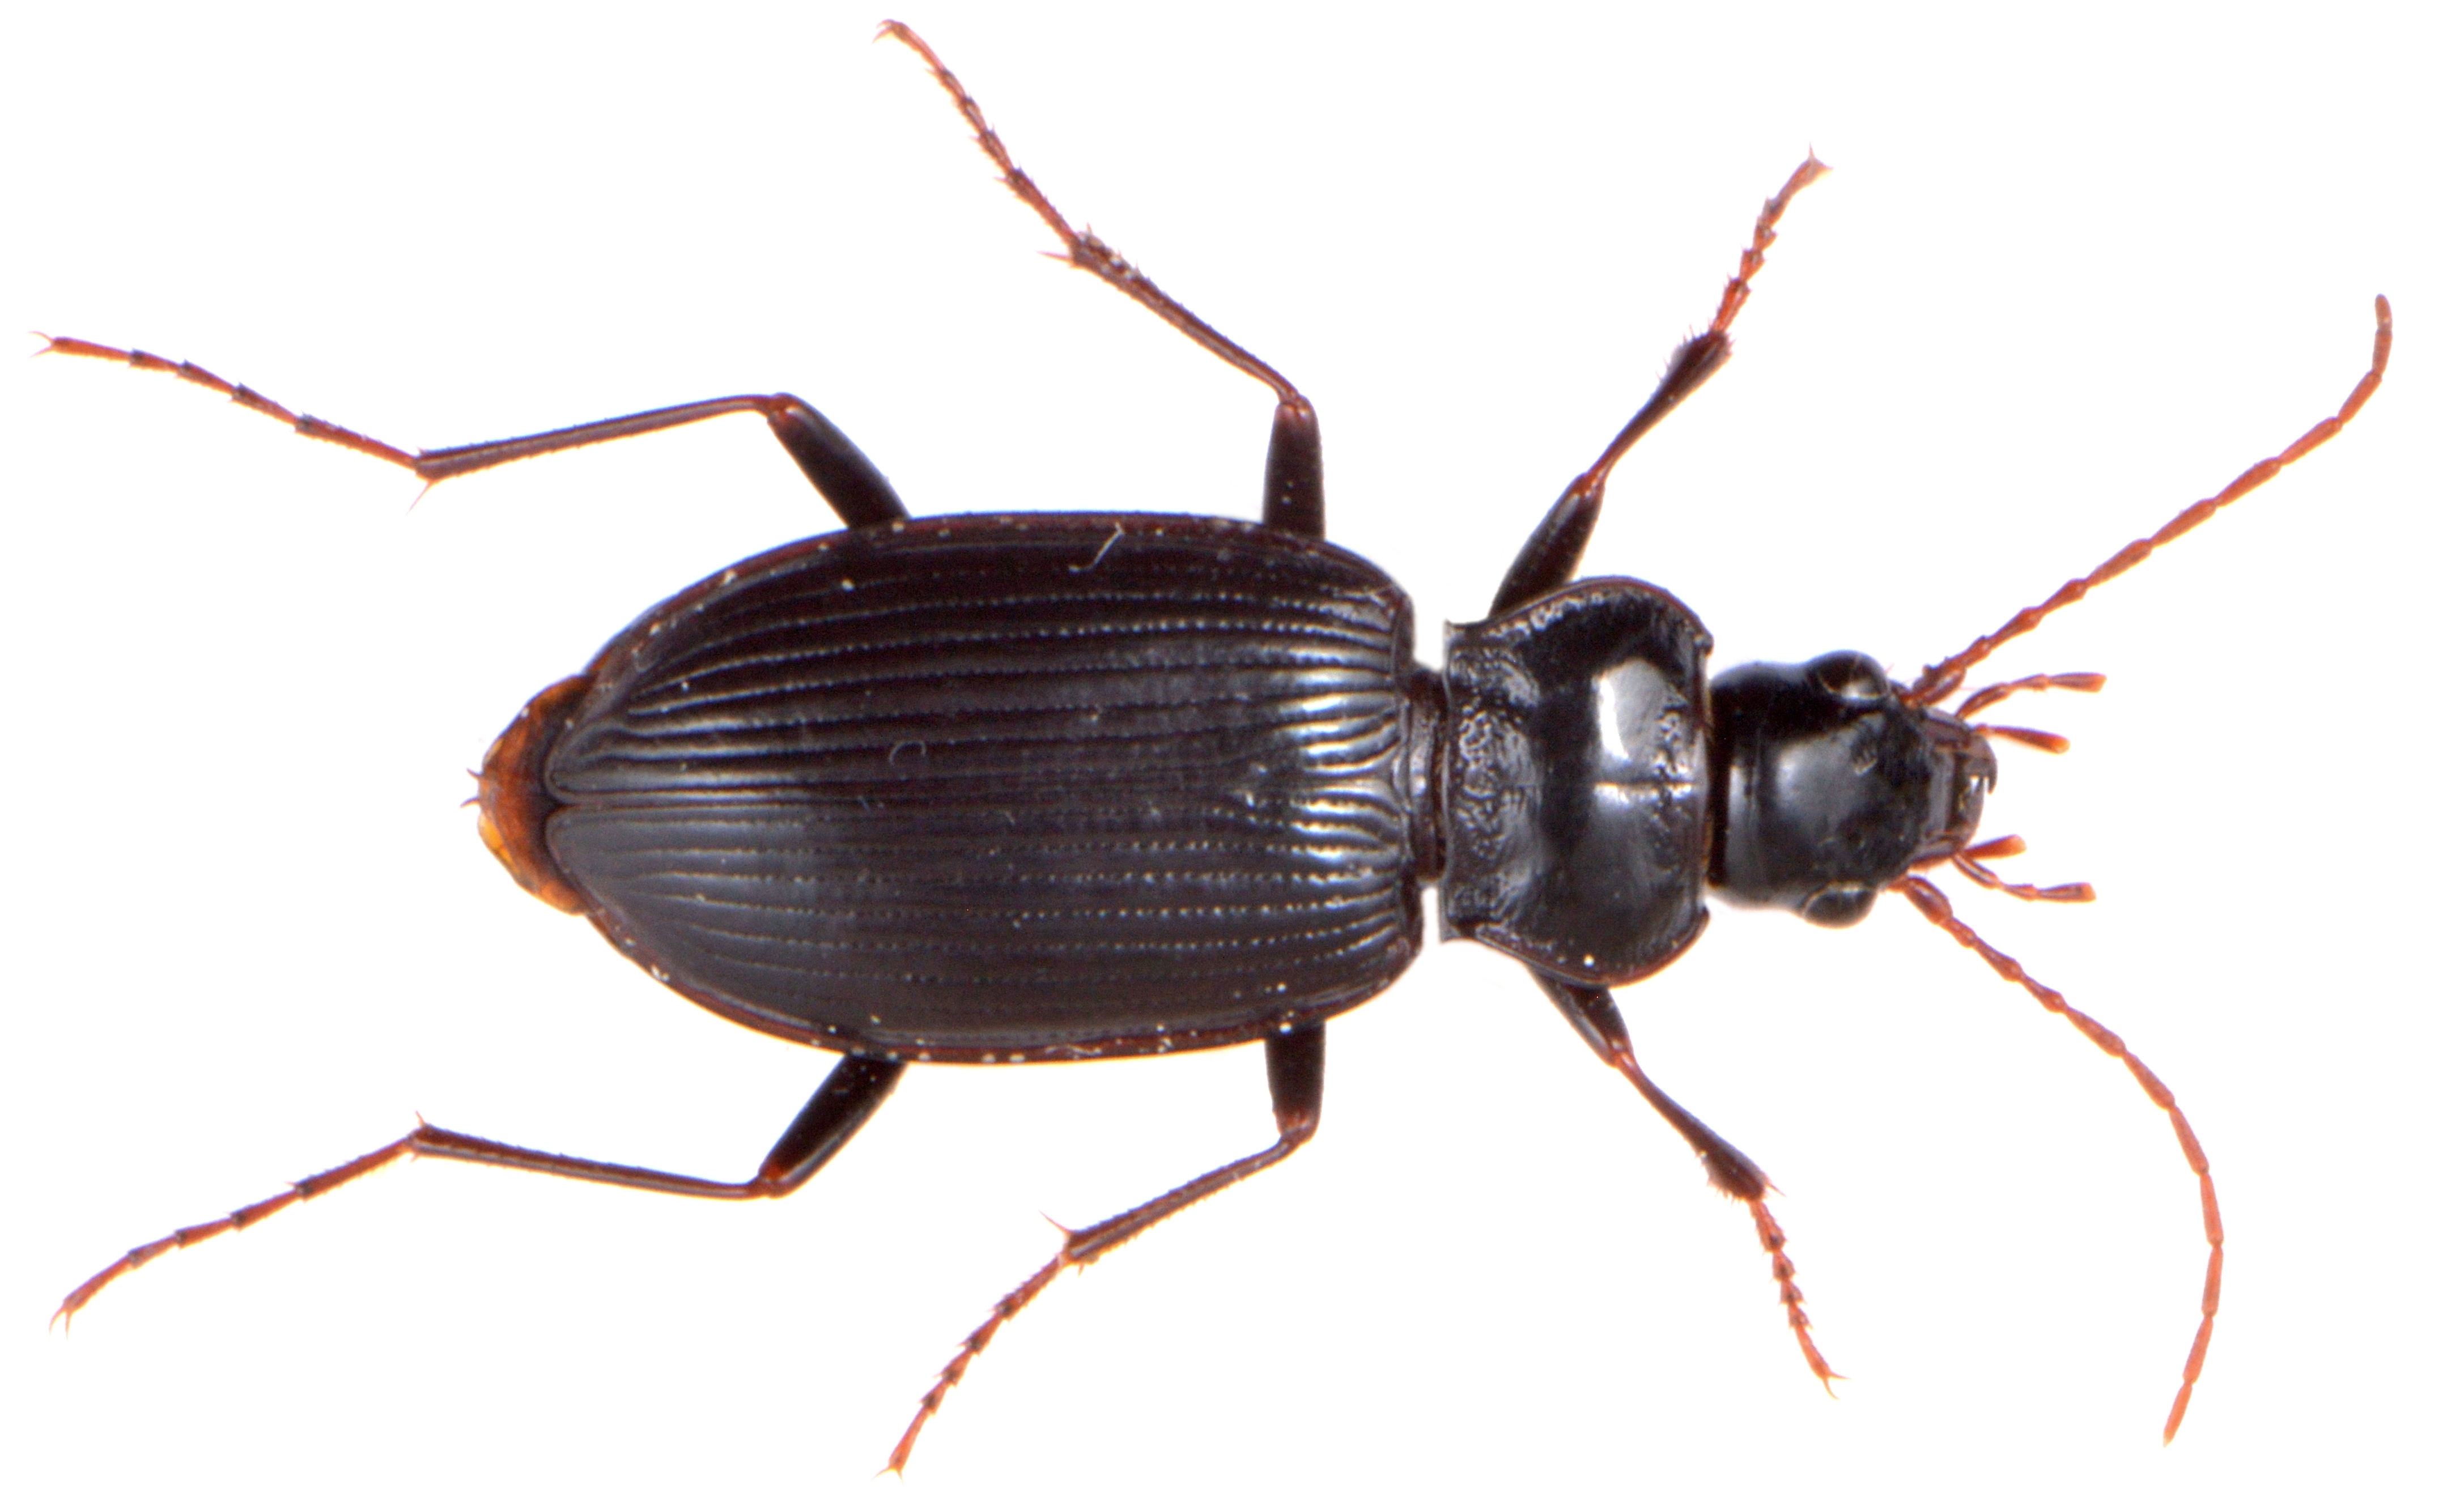
\includegraphics[width=\hsize]{src/figures/nebria.jpeg}
        \label{fig:nebria}
    \end{subfigure}
    % ~
    % \begin{subfigure}[t]{0.4\linewidth}
    %     \caption{}
    %     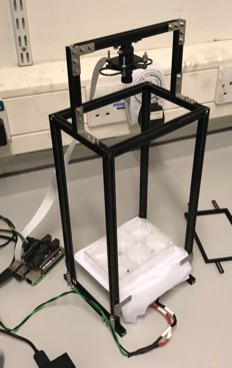
\includegraphics[width=\hsize]{src/figures/setup.jpg}
    %     \label{fig:setup}
    % \end{subfigure}
    % \newline
    \begin{subfigure}[t]{0.3\linewidth}
        \caption{}
        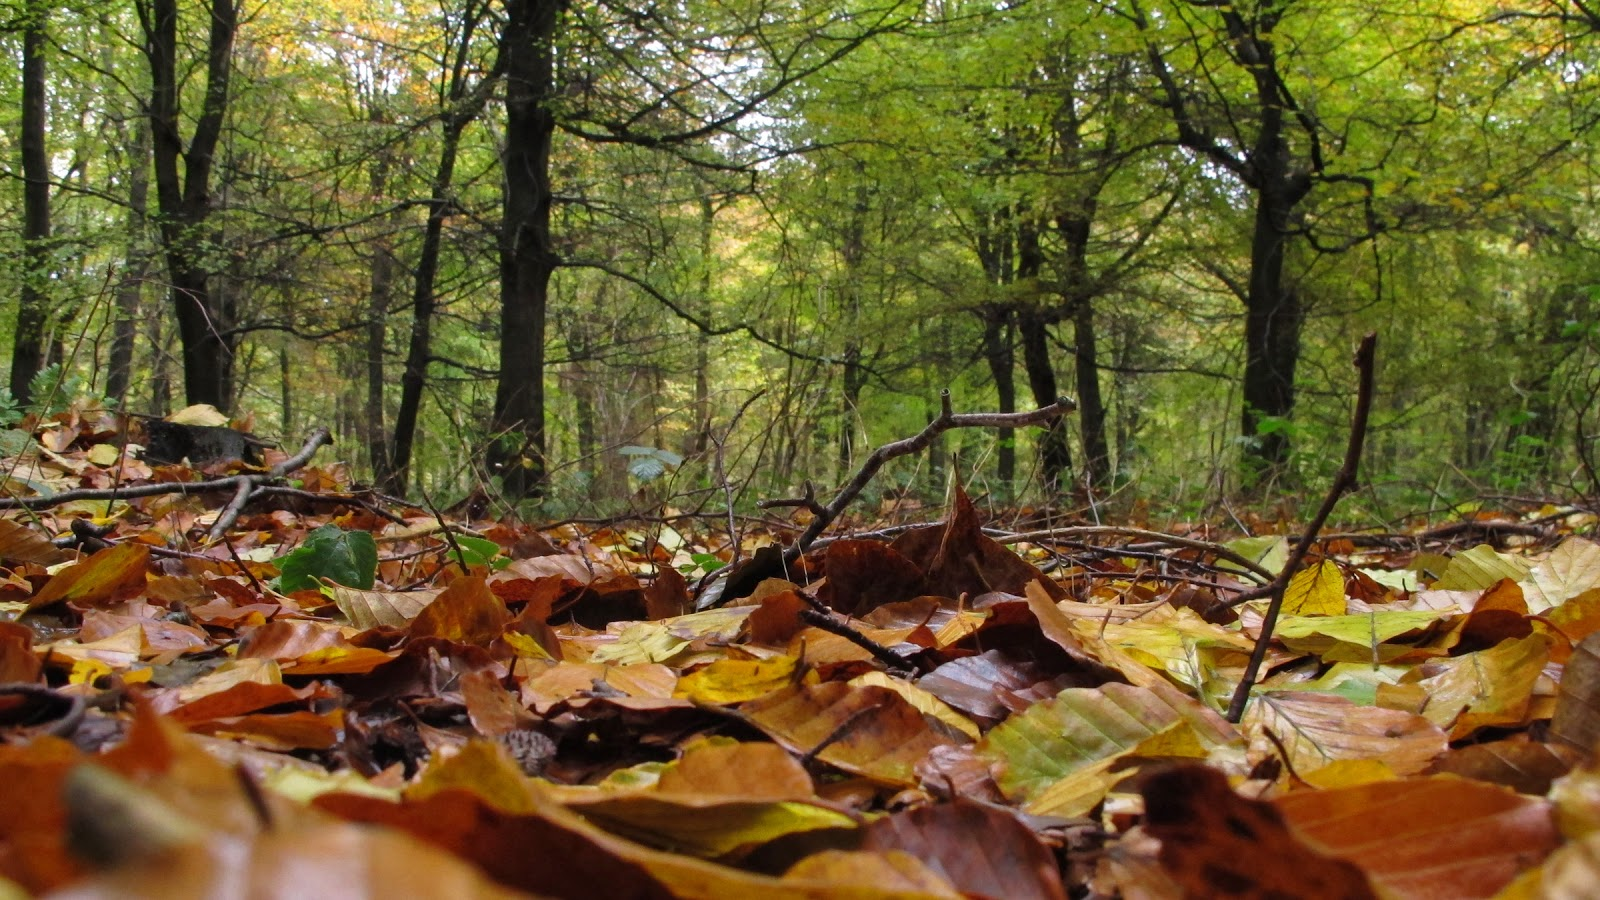
\includegraphics[width=\hsize]{src/figures/leaf-litter.jpeg}
        \label{fig:forest}
    \end{subfigure}
    \newline
    \begin{subfigure}[t]{0.3\linewidth}
        \caption{}
        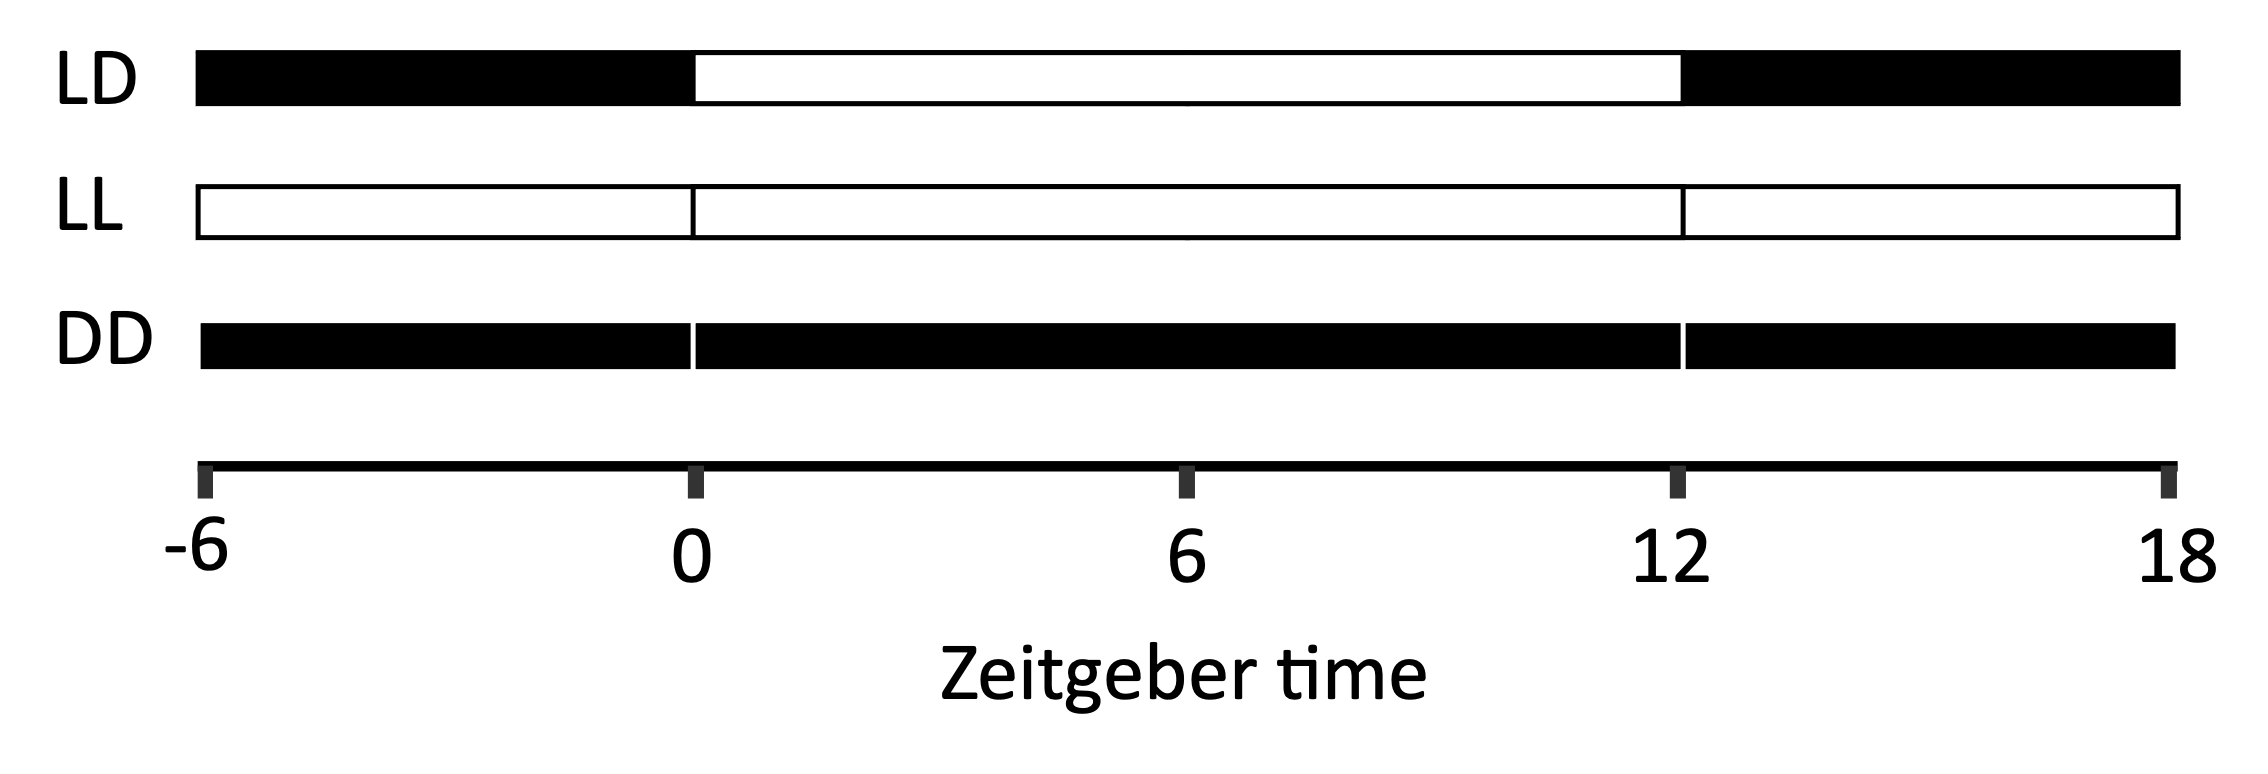
\includegraphics[width=\hsize]{src/figures/light-conditions.png}
        \label{fig:light-conditions}
    \end{subfigure}

    \caption{\textbf{Experimental setup and light conditions.} A) Beetles are placed in a 6-well plate, being recorded by an infrared camera mounted vertically above the plate. The plate is illuminated by infrared light from beneath, through a piece of diffusive fabric. B) Shows the time course of the the different light conditions used in the experiments.}
\end{figure}

% gradual light/dark (gLD), as aLD but with changes in light intensity happening over 30 minutes; 
% Make figure showing the lighting conditions

% (\cref{fig:conditions})

% \begin{figure}
%     \centering
%     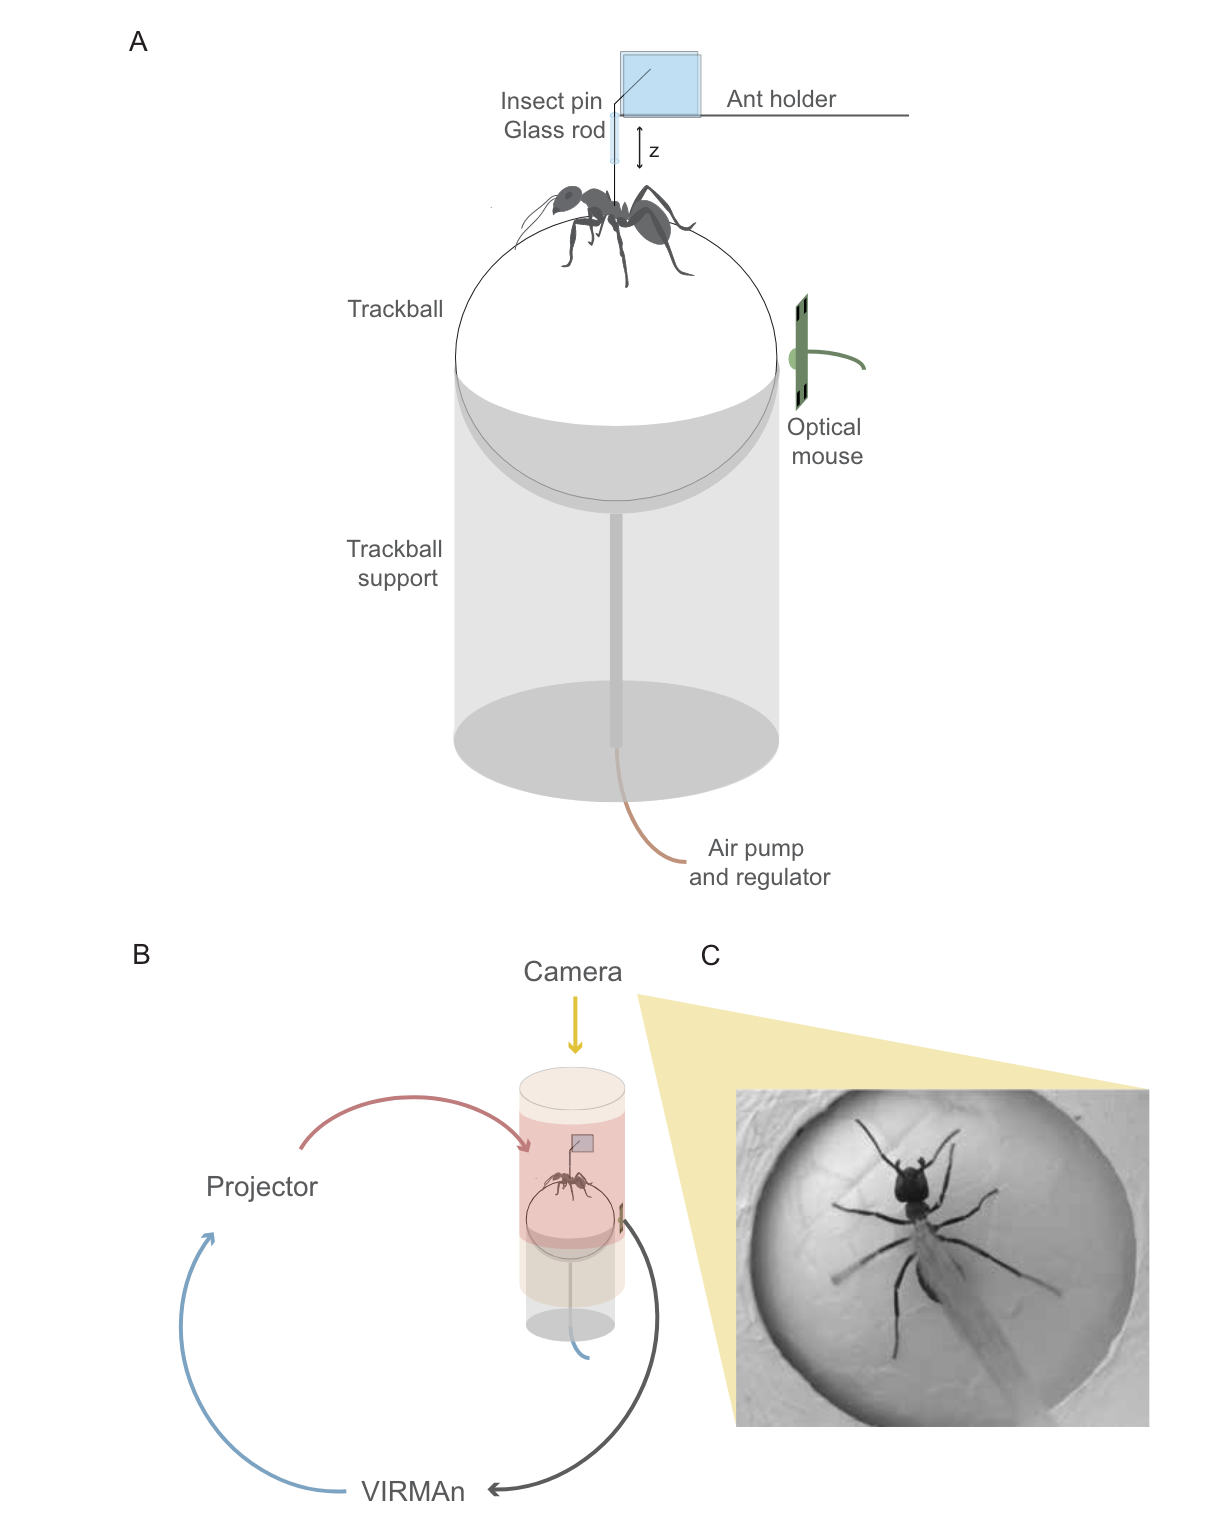
\includegraphics[width=\hsize]{src/figures/setup.png}
%     \caption{}
%     \label{fig:conditions}
% \end{figure}

% \subsection{Electrophysiology}
% Electroretinograms (ERG), local field potentials (LFP).

\subsection{Analysis}
Videos were recorded at 30fps as \lstinline{h.264} files and subsequently converted with to \lstinline{MPEG4} using ffmpeg, and tracked using TRex \citep{Walter2021a}. 
% The size of beetles was measured from individual frames from the recorded videos in ImageJ. \\
All data preprocessing was done in R and RStudio. A custom R package was developed, \{sleeprex\}, to analyse the relevant movement metrics. Each video was quality controlled to ensure that only good tracks were included and were attributed to the correct animal. Simultaneously obtained data from a light sensor was aligned and integrated to determine the light-on and -off times. This was then used to align all experiments to the light-on time. Subsequently, the data was down-sampled to allow further analysis. All plots were made with the \{ggplot2\} package.

% \sidenote{What the trex.R script does}
% \sidenote{What the sleepr-analysis scripts do. Maybe just a whole flow chart of the analysis pipeline}
% \sidenote{citation}.





